%%%%%%%%%%%%%%%%%%%%%%%%%%%%%%%%%%%%%%%%%%%%%%%%%%%%%%%%%%%%%%%%%%%%%%%%%%%%%%%%%%%%%%%%%%
\section{Use Case, Resources and Early-stage Results} \label{sect:motivation}            %
%%%%%%%%%%%%%%%%%%%%%%%%%%%%%%%%%%%%%%%%%%%%%%%%%%%%%%%%%%%%%%%%%%%%%%%%%%%%%%%%%%%%%%%%%%

In this section, we briefly discuss core use cases for the ApiNATOMY application: the generation of interactive schematics in support of genomics and drug discovery studies. In so doing, we introduce (i) some of the key ontological and data resources required in this case, as well as (ii) early-stage results of the ApiNATOMY application effort.

The domains of genomics and drug discovery are dependent on physiology knowledge, as both domains take into account the manufacture of gene products in different parts of the body and the regulated long-distance transport of molecules that interact with these products (e.g. drugs, nutrients, or gene products). The location of gene product manufacture (i.e. gene expression data, such as~\cite{EBI}), as well as routes associated with pharmacokinetic modeling of molecular interactors (drawn from resources such as~\cite{HMC+13}) may be usefully depicted in the form of a physiology \emph{circuitboard}.

In ApiNATOMY, a physiology circuitboard schematic consists of a combination of (i) an anatomical treemap and (ii) an overlay of process graphs. In our earlier prototypes (described in~\cite{BGS12,KBK14}), templates were applied to constrain the layout of tiles in treemaps of the Foundational Model of Anatomy (FMA)~\cite{RM03} ontology, such that nesting of one tile inside another indicates that the term asscoiated with the child tile is either a mereotopological \emph{part} or a \emph{subclass} of the term associated with the parent tile. 

In the following sections, we discuss our early-stage results in the construction of an ApiNATOMY Graphical User Interface (GUI) that supports user interaction with the circuitboard via point-and-click navigation of the treemap content. This type of interaction extends to also to involve process graphs. We arrange data in a hierarchical structure, starting from the upper level views of external and internal surfaces and organs. This upper level is arranged to resemble the longitudinal section through the middle of the human body (\cref{fig:tilemap-cylinder}).
Each of the organs in the plan is composed of multiple tissues and sub-organs, the structural information about them is obtained from the FMA ontology~\cite{RM03}. The GUI tool supports data filtering across multiple levels and contextual zooming into selected areas.

In addition, we report on the graphical projection of routes of (i) blood flow processes linking different regions of the human body (using data generated in~\cite{deB11}), as well as (ii) transport processes along neurons of the central nervous system (i.e. brain and spinal cord) with data obtained via the Neuroscience Information Framework~\cite{Gar+08}. The ApiNATOMY GUI is built from inception as a three dimensional (3D) environment. This facilitates interaction not only with 3D renderings of the circuit boards themselves, but also with a wide range of geometry/mesh formats for volumetric models of biological structure across scales. For instance, it is already possible to overlay Wavefront .obj data from BodyParts3D~\cite{MFT+09} as well as SWC data provided by neuromorpho.org~\cite{Asc06}. The management of such data is critical to the understanding of long-range molecular processes in genomics and drug discovery research.
% TODO: acknowledge the contribution of SharkViewer to our rendering of .swc files
% Sharkviewer: https://github.com/JaneliaSciComp/SharkViewer
% Janelia Farm research campus: http://www.janelia.org
% SWC File Format Specification: http://research.mssm.edu/cnic/swc.html
% I have asked the SharkViewer people how they'd like to be cited: https://github.com/JaneliaSciComp/SharkViewer/issues/4

In particular, we discuss our results in:
\begin{itemize}
  \item constraining of treemap layouts to generate stable anatomical treemaps,
  \item designing and overlaying physiological communication routes for the cardiovascular and neural systems, and
  \item querying and depicting of protein architecture diagrams for the anatomical overview of gene expression data and mathematical models relevant to molecular mechanisms.
\end{itemize}

\begin{figure}%
	\centering%
	\begin{minipage}[b]{.52\linewidth}
		\centering%
		\subfigure[Initial view of ApiNATOMY]{
			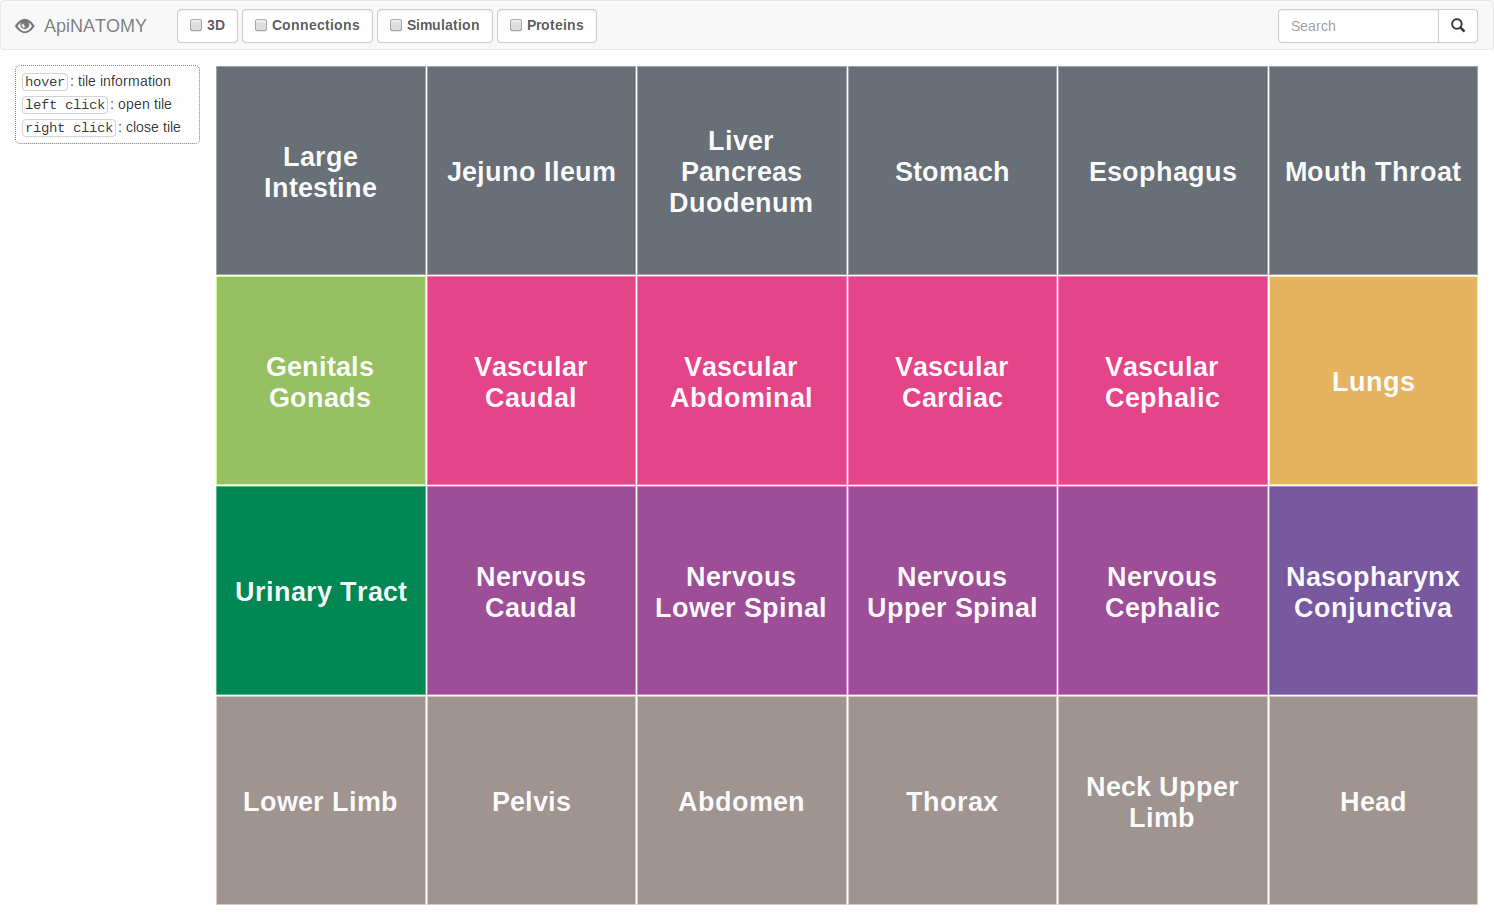
\includegraphics[width=\linewidth]{images/screenshot-main.png}
			\label{fig:24tiles}
		}
	\end{minipage}\hskip4mm
	\begin{minipage}[b]{.44\linewidth}
		\centering%
		\subfigure[Longitudinal section through the male human body, justifying the layout]{
			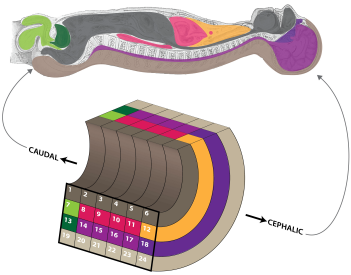
\includegraphics[width=\linewidth]{images/tilemap-cylinder.png}
			\label{fig:tilemap-cylinder}
		}
	\end{minipage}\vskip2mm
	\caption{The main 24-tile layout of the ApiNATOMY circuitboard}
	\label{fig:treemaps}
\end{figure}

%%%% Replaced by the figure above
%\begin{figure}
%	\centering
%	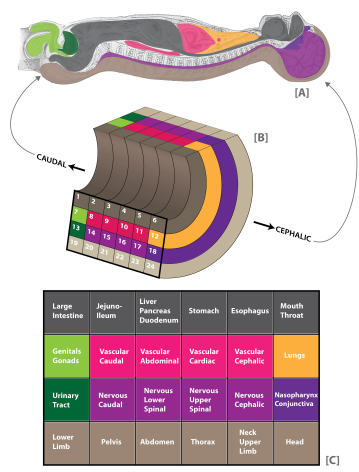
\includegraphics[width=6cm]{images/application.png}
%	\caption{Longitudinal section through the middle of the male human body}
%	\label{fig:application}
%\end{figure}
%	\subfigure[Visualizing medical ontologies using treemaps]{
%		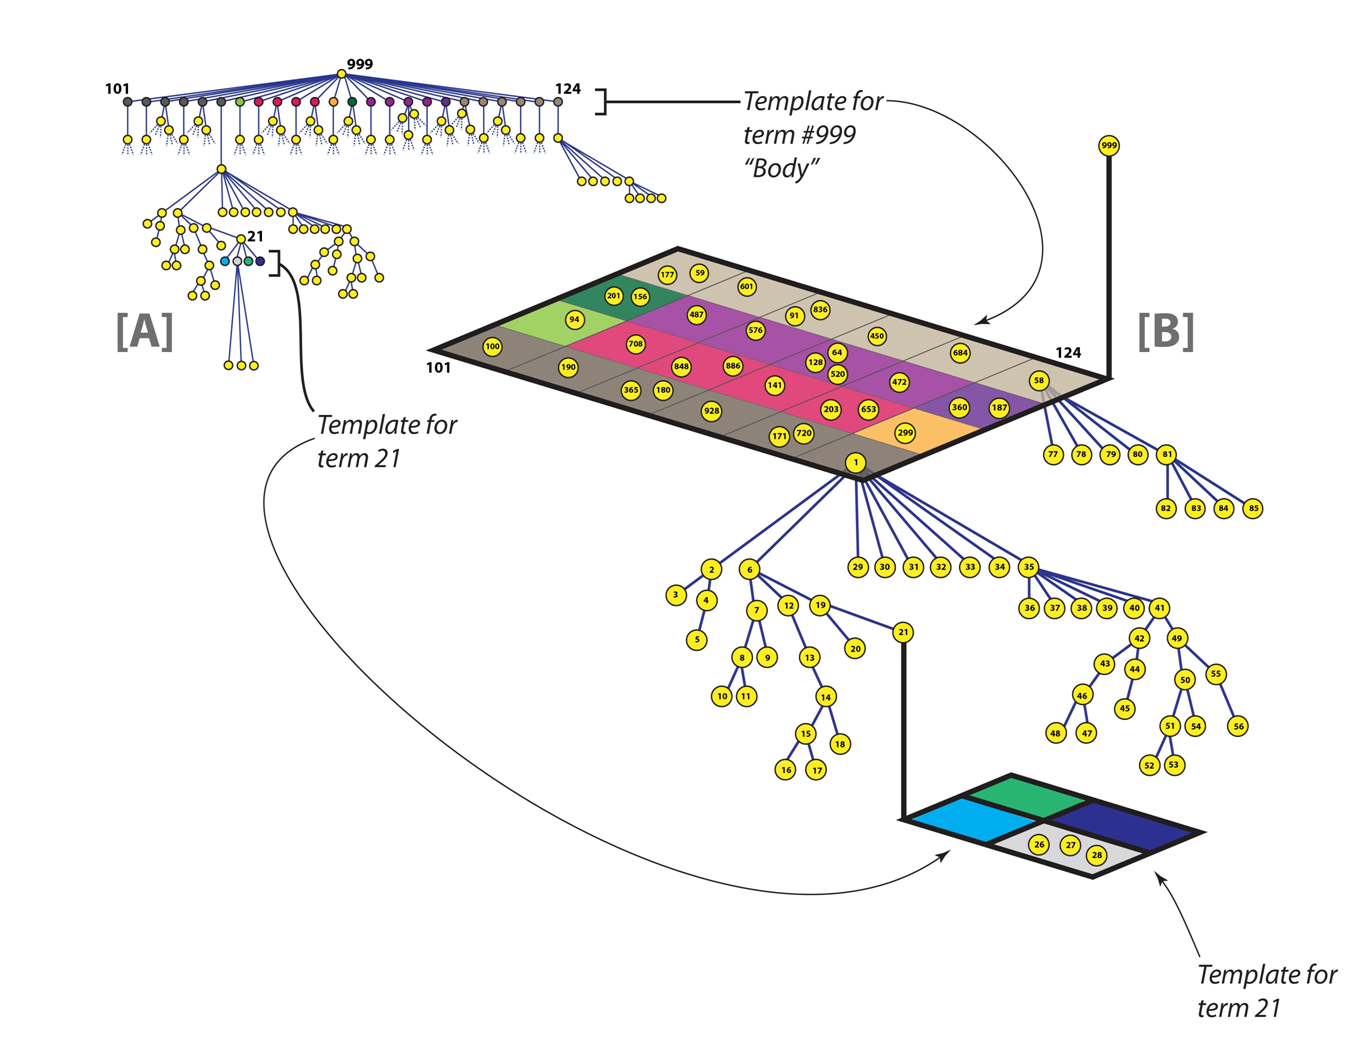
\includegraphics[width=7.3cm]{images/application1.png}
%	}


% TODO: refer to other figure
